\documentclass[12pt]{article}
\usepackage{mathtools,amssymb, amsthm, tikz}
\usepackage{tikz-3dplot}
\usetikzlibrary{angles, quotes}
\usetikzlibrary{patterns}
\usepackage[margin=1in]{geometry}
\usepackage{url}
\usepackage{natbib}
\usepackage[colorlinks=true, linkcolor=black, urlcolor=blue, citecolor=blue]{hyperref}
\usepackage[T1]{fontenc}
\usepackage[utf8]{inputenc}
\usepackage{lmodern}
\usepackage{fontspec}
\setmainfont{Times New Roman}

\title{Edge Function}
\author{Pintér Bálint}
\renewcommand{\contentsname}{Tartalomjegyzék}
\renewcommand{\bibsection}{\section*{Források}}
\newcommand{\paralelogramma}{
    
\begin{tikzpicture}[scale=0.15, baseline=(current bounding box.center)]
        \draw[black] (0,0) -- (1.5,0) -- (2.3,1) -- (0.8,1) -- cycle;
    \end{tikzpicture}
}
\tdplotsetmaincoords{60}{130}

\begin{document}
\maketitle
\newpage
\tableofcontents
\newpage

\section{Bevezetés}
Az edge function egy lineáris függvény, amellyel egy egyenessel kettéosztott
síkon lévő pontokat lehet három régióba osztani:
\begin{itemize}
    \item Az egyenestől `jobbra' lévő pontok (ahol a függvény értéke pozitív).
    \item Az egyenestől `balra' lévő pontok (ahol a függvény értéke negatív).
    \item Az egyenesre illeszkedő pontok (ahol a függvény értéke nulla).
\end{itemize}
\begin{center}
    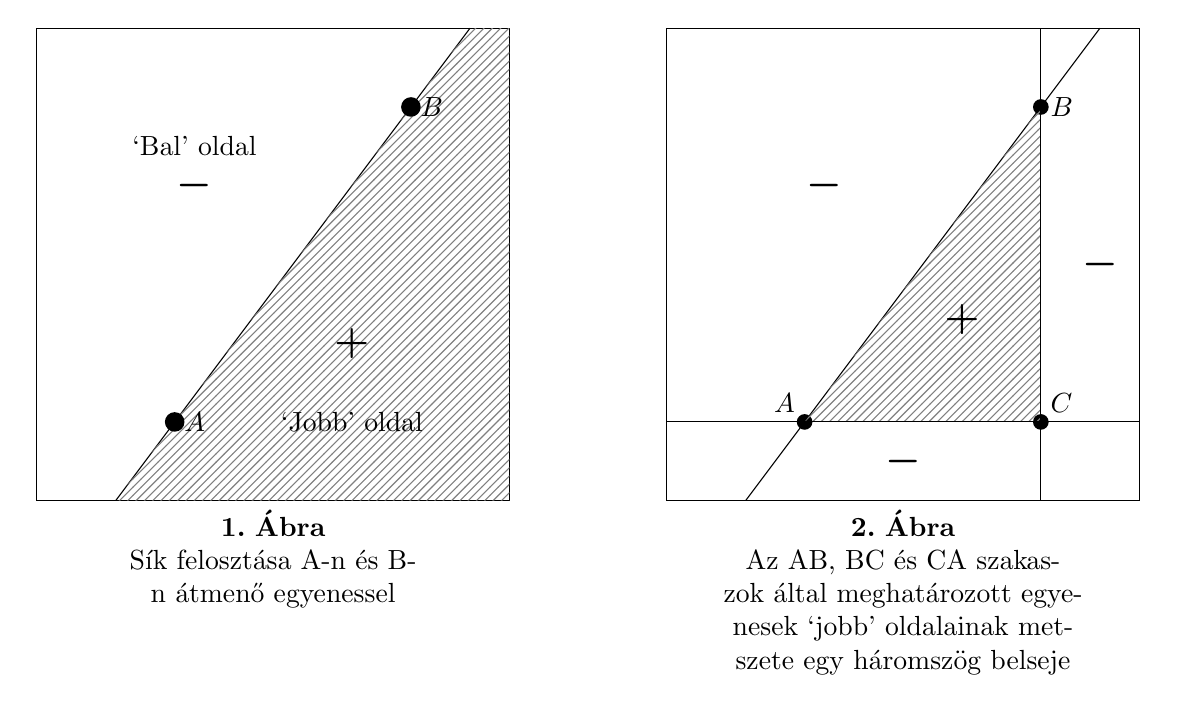
\begin{tikzpicture}
        \coordinate (BL1) at (0,0);
        \coordinate (BR1) at (6,0);
        \coordinate (TR1) at (6,6);
        \draw (BL1) rectangle (TR1);
        \coordinate (B1) at (1,0);
        \coordinate (T1) at (5.5,6);
        \draw (B1) -- (T1);
        \fill[pattern=north east lines, pattern color=gray]
        (T1) -- (TR1) -- (BR1) -- (B1) -- cycle;

        \coordinate (A1) at (1.75,1);
        \node[circle, fill, inner sep=2.5pt] at (A1) {};

        \coordinate (B1) at (4.75,5);
        \node[circle, fill, inner sep=2.5pt] at (B1) {};

        \node[right] at (A1) {$A$};
        \node[right] at (B1) {$B$};
        \node[font=\Large] at (2,4) {$\boldsymbol{-}$};
        \node[] at (2,4.5) {`Bal' oldal};
        \node[font=\Large] at (4,2) {$\boldsymbol{+}$};
        \node[] at (4, 1) {`Jobb' oldal};
        \node[below, text width=6cm, align=center] at (3,0) {\textbf{1.~Ábra}\\Sík felosztása A-n és B-n átmenő egyenessel};

        \coordinate (BL2) at (8,0);
        \coordinate (BR2) at (14,0);
        \coordinate (TR2) at (14,6);
        \draw (BL2) rectangle (TR2);
        \coordinate (B2) at (9,0);
        \coordinate (T2) at (13.5,6);
        \draw (B2) -- (T2);

        \coordinate (A2) at (9.75,1);
        \node[circle, fill, inner sep=2pt] at (A2) {};

        \coordinate (B2) at (12.75,5);
        \node[circle, fill, inner sep=2pt] at (B2) {};

        \coordinate (C2) at (12.75,1);
        \node[circle, fill, inner sep=2pt] at (C2) {};
        \draw (A2) -- (C2) -- (B2);
        \fill[pattern=north east lines, pattern color=gray]
        (A2) -- (B2) -- (C2) -- cycle;

        \draw (12.75,6) -- (12.75,0);

        \draw (8,1) -- (14,1);

        \node[font=\Large] at (10,4) {$\boldsymbol{-}$};

        \node[font=\Large] at (13.5,3) {$\boldsymbol{-}$};

        \node[font=\Large] at (11,0.5) {$\boldsymbol{-}$};

        \node[font=\Large] at (11.75,2.3) {$\boldsymbol{+}$};

        \node[above left] at (A2) {$A$};
        \node[right] at (B2) {$B$};
        \node[above right] at (C2) {$C$};
        \node[below, text width=6cm, align=center] at (11,0) {\textbf{2.~Ábra}\\Az AB, BC és CA szakaszok által meghatározott egyenesek `jobb' oldalainak metszete egy háromszög belseje};

    \end{tikzpicture}
\end{center}
A 2. ábra szemlélteti, hogy a háromszög `belseje' a három oldalhoz tartozó megfelelő irányú edge function előjelei alapján meghatározható. Ezt használjuk 3D renderelésben, hogy a pixelt (pontot) tartalmazza-e a háromszög.
\newpage
\section{Edge function levezetése}
\begin{itemize}
    \item Legyen a szakasz kezdőpontja $P_{0} = (X,Y)$
    \item Legyen a szakasz végpontja $P_{1} = (X + dX,Y + dY)$
          \begin{itemize}
              \item Ekkor a $\vec{P_{0}P_{1}}=\vec{v}=((X + dX) - X, (Y + dY) - Y)=(dX, dY)$
          \end{itemize}
    \item Legyen a vizsgált pont $P = (x,y)$
          \begin{itemize}
              \item Ekkor a $\vec{P_{0}P}=\vec{u}=(x - X, y - Y)$
          \end{itemize}
\end{itemize}
Az edge function lényegében a két vektor által alkotott $2 \times 2$-es mátrix determinánsa.
\begin{align*}
    \det
    \begin{bmatrix}
        u_{x} & u_{y} \\
        v_{x} & v_{y}
    \end{bmatrix} & =u_{x}v_{y}-u_{y}v_{x}\quad\text{/ } \det
    \begin{bmatrix}
        a & b \\
        c & d
    \end{bmatrix}=ad-bc
\end{align*}
Helyettesítsük be az értékeinket:
\begin{align*}
    u_{x} & = x - X \\
    u_{y} & = y - Y \\
    v_{x} & = dX    \\
    v_{y} & = dY    \\
\end{align*}
A végeredmény:
\begin{align*}
    E(x,y)            & = (x - X)dY-(y - Y)dX \\
    E_{P_{0}P_{1}}(P) & = (x - X)dY-(y - Y)dX
\end{align*}
\newpage
\section{Edge function működési elve}
\subsection{Edge function geometriai jelentése}
A determináns előjele $2\times2$-es mátrix esetén:
\begin{itemize}
    \item Pozitív esetben a vektorok jobbsodrású (pozitív irányítású) rendszert alkotnak.
    \item Negatív esetben a vektorok balsodrású (negatív irányítású) rendszert alkotnak.
    \item Nulla esetén párhuzamosak.
\end{itemize}
A determináns abszolút értéke $2\times2$-es mátrix esetén a mátrix sorvektorai által kifeszített paralelogramma területét jelenti. Így, ha ezt elosztjuk kettővel, akkor megkapjuk a háromszög területét. 
\begin{center}
    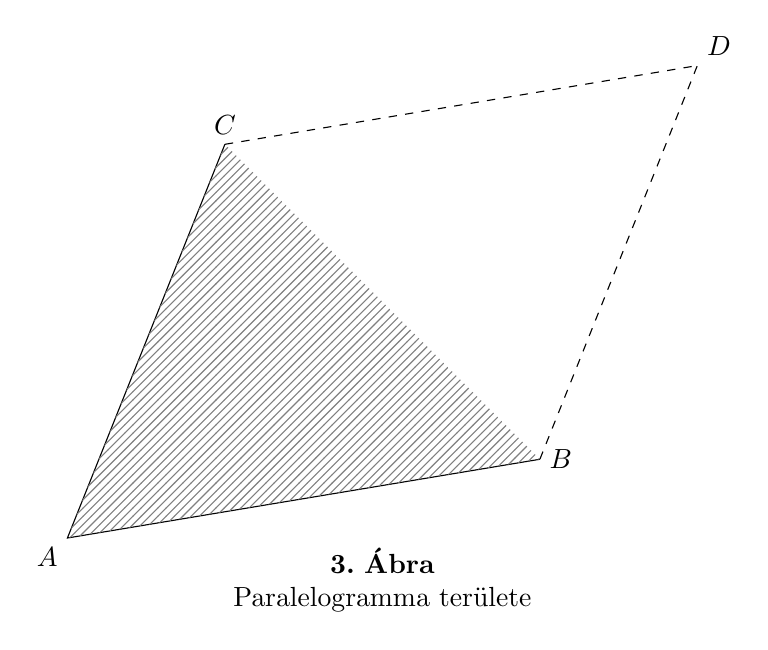
\begin{tikzpicture}

        \coordinate (A) at (0,0);
        \coordinate (B) at (6,1);

        \coordinate (C) at (2,5);
        \coordinate (D) at (8,6);
        \draw (C) -- (A) -- (B);
        \draw[dashed] (B) -- (D);
        \draw[dashed] (C) -- (D);
        \fill[pattern=north east lines, pattern color=gray]
        (A) -- (B) -- (C) -- cycle;

        \node[below left] at (A) {$A$};
        \node[right] at (B) {$B$};
        \node[above] at (C) {$C$};
        \node[above right] at (D) {$D$};
        \node[below, text width=6cm, align=center] at (4,0) {\textbf{3.~Ábra}\\Paralelogramma területe};
    \end{tikzpicture}
    \begin{align*}
        E_{AC}(B)            & =T_{ABCD_{\paralelogramma}} \\
        \frac{1}{2}E_{AC}(B) & =T_{ABC_{\Delta}}
    \end{align*}
\end{center}
\subsubsection{Baricentrikus koordináták}
Az előbb kiszámolt területet felhasználjuk a háromszögön belüli pont (pixel) baricentrikus koordinátáinak kiszámolására (A baricentrikus koordinátákkal tudjuk interpolálni a háromszög egy belső pontjára a háromszög csúcsaihoz vett értékeket).
\begin{center}
    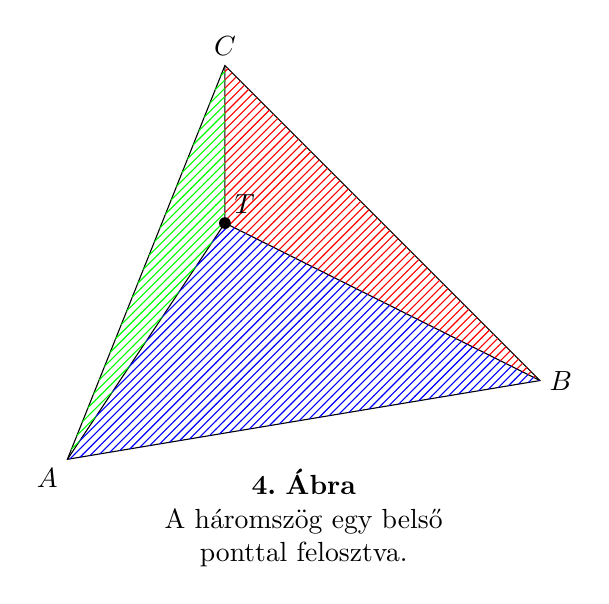
\begin{tikzpicture}

        \coordinate (A) at (0,0);
        \coordinate (B) at (6,1);

        \coordinate (C) at (2,5);
        \coordinate (T) at (2,3);
        \draw (A) -- (B) -- (C) -- cycle;
        \draw (A) -- (T) -- (C);
        \draw (T) -- (B);
        \fill[pattern=north east lines, pattern color=green]
        (A) -- (T) -- (C) -- cycle;
        \fill[pattern=north east lines, pattern color=red]
        (B) -- (T) -- (C) -- cycle;
        \fill[pattern=north east lines, pattern color=blue]
        (A) -- (T) -- (B) -- cycle;

        \node[circle, fill, inner sep=1.5pt] at (T) {};

        \node[below left] at (A) {$A$};
        \node[right] at (B) {$B$};
        \node[above] at (C) {$C$};
        \node[above right] at (T) {$T$};
        \node[below, text width=6cm, align=center] at (3,0) {\textbf{4.~Ábra}\\A háromszög egy belső ponttal felosztva.};
    \end{tikzpicture}
    \begin{align*}
        \textcolor{red}{\lambda_{A}}                                                              & =\frac{T_{TBC_{\textcolor{red}{\Delta}}}}{T_{ABC_{\Delta}}}   & \text{/ } T_{TBC_{\textcolor{red}{\Delta}}}=\frac{1}{2}E_{CB}(T)   \\
        \textcolor{green}{\lambda_{B}}                                                            & =\frac{T_{ATC_{\textcolor{green}{\Delta}}}}{T_{ABC_{\Delta}}} & \text{/ } T_{ATC_{\textcolor{green}{\Delta}}}=\frac{1}{2}E_{AC}(T) \\
        \textcolor{blue}{\lambda_{C}}                                                             & =\frac{T_{ATB_{\textcolor{blue}{\Delta}}}}{T_{ABC_{\Delta}}}  & \text{/ } T_{ATB_{\textcolor{blue}{\Delta}}}=\frac{1}{2}E_{BA}(T)  \\
                                                                                                  & \text{Fontos tulajdonságuk:}                                  &                                                                    \\
        \textcolor{red}{\lambda_{A}}+\textcolor{green}{\lambda_{B}}+\textcolor{blue}{\lambda_{C}} & =1                                                            & \text{/ Területszámítás axiómáiból is következik}
    \end{align*}
\end{center}
\subsection{Vektoriális szorzatos magyarázat}
A vektoriális szorzat definíció szerint csak háromdimenziós vektorokra van
értelmezve. Ha azonban a $\vec{u}$ és $\vec{v}$ vektorainkat kiegészítjük $z=0$
koordinátával, akkor az így kapott két vektor vektoriális szorzatának a $z$
koordinátája az edge function értéke.

\begin{center}
    \begin{minipage}[t]{0.48\textwidth}
        \centering
        \begin{tikzpicture}[tdplot_main_coords,scale=1.5, line cap=round]
            \begin{scope}[canvas is xy plane at z=0]
                \draw[step=0.5, gray!30, very thin] (-1.5,-1.5) grid (1.5,1.5);
                \draw[thick] (-1.5,0) -- (1.5,0);
                \draw[thick] (0,-1.5) -- (0,1.5);
            \end{scope}
            \coordinate (O) at (0,0,0);
            \coordinate (A) at (-1,0,0);
            \tdplotsetcoord{B}{-1}{90}{0}
            \pgfmathsetmacro{\Cz}{-sin(0)}
            \coordinate (C) at (0, 0,\Cz);
            \draw[->, red, ultra thick] (O) -- (A) node[anchor=north east] {$\vec{v}$};
            \draw[->, blue, ultra thick] (O) -- (B) node[anchor=south west] {$\vec{u}$};
            \draw[->, green!80!black, ultra thick] (O) -- (C) node[anchor=south west] {$\mathbf{z}$};
        \end{tikzpicture}
        \vspace{0.5ex}
        \hspace*{4mm}$z = 0\Rightarrow$ \\ Párhuzamos a két vektor \\ A pont a vonalon van
    \end{minipage}%
    \hfill
    \begin{minipage}[t]{0.48\textwidth}
        \centering
        \begin{tikzpicture}[tdplot_main_coords,scale=1.5, line cap=round]
            \begin{scope}[canvas is xy plane at z=0]
                \draw[step=0.5, gray!30, very thin] (-1.5,-1.5) grid (1.5,1.5);
                \draw[thick] (-1.5,0) -- (1.5,0);
                \draw[thick] (0,-1.5) -- (0,1.5);
            \end{scope}
            \coordinate (O) at (0,0,0);
            \coordinate (A) at (-1,0,0);
            \tdplotsetcoord{B}{-1}{90}{90}
            \pgfmathsetmacro{\Cz}{-sin(90)}
            \coordinate (C) at (0, 0,\Cz);
            \draw[->, red, ultra thick] (O) -- (A) node[anchor=north east] {$\vec{v}$};
            \draw[->, blue, ultra thick] (O) -- (B) node[anchor=south west] {$\vec{u}$};
            \draw[->, green!80!black, ultra thick] (O) -- (C) node[anchor=south west] {$\mathbf{z}$};
        \end{tikzpicture}
        \vspace{0.5ex}
        \hspace*{4mm}$z < 0\Rightarrow$ \\ A pont `balra' van a vonaltól
    \end{minipage}

    \vspace{1cm}
    \begin{minipage}[t]{0.48\textwidth}
        \centering
        \begin{tikzpicture}[tdplot_main_coords,scale=1.5, line cap=round]
            \begin{scope}[canvas is xy plane at z=0]
                \draw[step=0.5, gray!30, very thin] (-1.5,-1.5) grid (1.5,1.5);
                \draw[thick] (-1.5,0) -- (1.5,0);
                \draw[thick] (0,-1.5) -- (0,1.5);
            \end{scope}
            \coordinate (O) at (0,0,0);
            \coordinate (A) at (-1,0,0);
            \tdplotsetcoord{B}{-1}{90}{180}
            \pgfmathsetmacro{\Cz}{-sin(180)}
            \coordinate (C) at (0, 0,\Cz);
            \draw[->, red, ultra thick] (O) -- (A) node[anchor=north east] {$\vec{v}$};
            \draw[->, blue, ultra thick] (O) -- (B) node[anchor=south west] {$\vec{u}$};
            \draw[->, green!80!black, ultra thick] (O) -- (C) node[anchor=south west] {$\mathbf{z}$};
        \end{tikzpicture}
        \vspace{0.5ex}
        $z = 0\Rightarrow$ \\ Párhuzamos a két vektor \\ A pont a vonalon van
    \end{minipage}
    \hfill
    \begin{minipage}[t]{0.48\textwidth}
        \centering
        \begin{tikzpicture}[tdplot_main_coords,scale=1.5, line cap=round]
            \begin{scope}[canvas is xy plane at z=0]
                \draw[step=0.5, gray!30, very thin] (-1.5,-1.5) grid (1.5,1.5);
                \draw[thick] (-1.5,0) -- (1.5,0);
                \draw[thick] (0,-1.5) -- (0,1.5);
            \end{scope}
            \coordinate (O) at (0,0,0);
            \coordinate (A) at (-1,0,0);
            \tdplotsetcoord{B}{-1}{90}{270}
            \pgfmathsetmacro{\Cz}{-sin(270)}
            \coordinate (C) at (0, 0,\Cz);
            \draw[->, red, ultra thick] (O) -- (A) node[anchor=north east] {$\vec{v}$};
            \draw[->, blue, ultra thick] (O) -- (B) node[anchor=south west] {$\vec{u}$};
            \draw[->, green!80!black, ultra thick] (O) -- (C) node[anchor=south west] {$\mathbf{z}$};
        \end{tikzpicture}
        \vspace{0.5ex}
        $z > 0\Rightarrow$ \\ A pont `jobbra' van a vonaltól
    \end{minipage}
    \textbf{5.~Ábra}\\Vektoriális szorzattal szemléltetve
\end{center}
\section{Inkrementalitás}
Mivel az edge function lineáris számolhatjuk inkrementálisan. Elég egyszer
kiszámolni mindegyik oldalra magát az edge functiont:
\[
    E(x,y) = (x - X)dY-(y - Y)dX
\]
Utána egy összeadással kiszámolhatjuk a többi pontokra (pixelekre) \\
A következő egyenletek képernyő térbeli koordináta-rendszerben vannak x jobbra nő, y lefele nő:
\begin{align*}
    E(x+1,y) & = E(x,y) + dY \\
    E(x-1,y) & = E(x,y) - dY \\
    E(x,y+1) & = E(x,y) - dX \\
    E(x,y-1) & = E(x,y) + dX
\end{align*}
Az edge function 5 műveletjét (3 kivonás, 2 szorzás), így lecsökkentjük egy műveletre (1 összeadás). Ez egy $1920\times1080$ felbontású képnél például jelentős mennyiségű műveletet jelent.
Használhatjuk egy adott $L$ távol lévő pixelre is.
\begin{align*}
    E(x+L,y) & = E(x,y) + L\times dY \\
    E(x-L,y) & = E(x,y) - L\times dY \\
    E(x,y+L) & = E(x,y) - L\times dX \\
    E(x,y-L) & = E(x,y) + L\times dX
\end{align*}
Bizonyítása egyik esetre:
\begin{align*}
    E(x+L,y) & = ((x+L) - X)dY-(y - Y)dX          &                                      \\
    E(x+L,y) & = (x - X + L)dY-(y - Y)dX          &                                      \\
    E(x+L,y) & = (x - X)dY + L\times dY-(y - Y)dX &                                      \\
    E(x+L,y) & = (x - X)dY-(y - Y)dX + L\times dY & \text{/ } E(x,y)=(x - X)dY-(y - Y)dX \\
    E(x+L,y) & = E(x,y) + L\times dY              &
\end{align*}
A többi esetet is hasonlóan lehet belátni.
\newpage
\nocite{*}
\bibliographystyle{plainnat}
\bibliography{forrasok}

\end{document}